 \chapter{\label{chap:intro}Discussão}
 
Os controles que tiveram a maior preocupação por parte dos desenvolvedores na seção de controle de acesso foram os que pertenciam ao objetivo de controle de gerenciamento de acesso de usuários e de controle de acesso ao sistema e â aplicação. Ao todo objetivo de controle 9.2 (Figura \ref{fig:cont}) teve 6 questões marcadas como uma preocupação (questões em verde), que pertenciam aos controles de política de controle de acesso, provisionamento para acesso de usuário e gerenciamento da informação de autenticação secreta de usuários e o objetivo de controle 9.4 (Figura \ref{fig:cont}) teve 4 questões marcadas como uma preocupação, que pertenciam aos controles de procedimentos seguros de entrada no sistema e sistema de gerenciamento de senha. 

\begin{figure}[H]
\centering
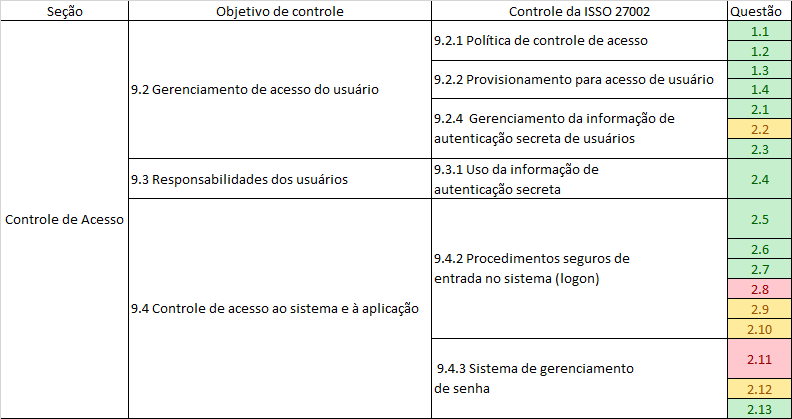
\includegraphics[scale=0.8]{fig2/controles1.png}
\caption{}
\label{fig:cont}
\end{figure}


O controles com maior preocupação por partes dos desenvolvedores na seção de criptografia era o de políticas para o uso de controle criptográfico que pertence ao objetivo de controle, "Controles criptográficos".

\begin{figure}[H]
\centering
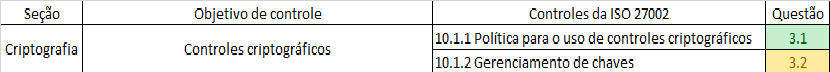
\includegraphics[scale=0.8]{fig2/controles2.png}
\caption{}
\label{fig:cont}
\end{figure}


Os controles que tiveram maior preocupação por parte dos desenvolvedores na de seção de "Segurança nas operações", pertencem aos aos objetivos de controle de "Responsabilidades e procedimentos operacionais" 
\begin{figure}[H]
\centering
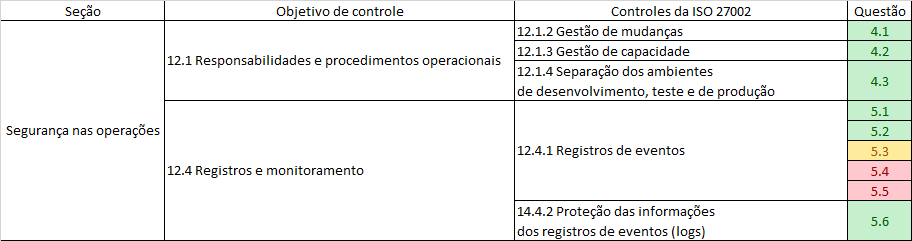
\includegraphics[scale=0.7]{fig2/controles3.png}
\caption{}
\label{fig:cont}
\end{figure}


\begin{figure}[H]
\centering
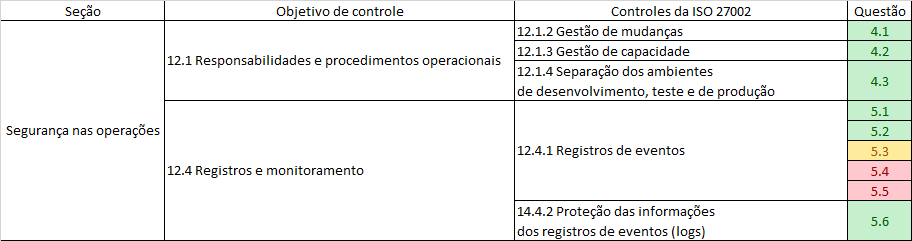
\includegraphics[scale=0.7]{fig2/controles3.png}
\caption{}
\label{fig:cont}
\end{figure}